\documentclass[12pt]{article}
\usepackage{amsmath, amsfonts}
\usepackage{graphicx}
\usepackage{tabularx}

\graphicspath{{./img}}
\usepackage[margin=1in]{geometry}

\usepackage{xeCJK}
\setCJKmainfont{WenQuanYi Micro Hei Mono}

\usepackage{algorithm}

\usepackage[backend=biber,style=ieee]{biblatex}
\addbibresource{report.bib}

\begin{document}
\title{Data Science Homework 4}
\author{Andr\'es Ponce,
\and
彭思安
\and
P76107116
}

\begin{document}
\maketitle
\section{Introduction}
Our data's properties will determine the pre-processing steps we take to ensure our 
model performs well with new data.
For instance, since machine learning methods can for the most part deal only with
numerical values, its is necessary to convert string-based values into numbers.
Such methods range from just assigning a numerical value to a class index to 
using hash tables to store indices of the column to which it belongs.

Another common issue in the data processing stage is imbalanced data.
This happens when some categories in our data happen less often than others,
sometimes much less often.
These categories are known as \textbf{minority class}, and more common
classes or categories are known as \textbf{majority class}.
To ensure our model is exposed to the category, we can either remove elements
from the majority class with \textbf{undersampling methods} or create new samples
from the minority class using \textbf{oversampling methods}.

In this assignment we investigate the relation between datasets and different
encoding and sampling methods.
First, we describe the datasets used, then conduct experiments on different
combinations of encoding and sampling methods.

\section{Datasets}
% Make the table here
% Plot the class imbalances
\begin{centering}
\begin{table}
\begin{tabular}{|c|c|c|c|c|c|}
	\hline
	Dataset & Features & Categorical & Numerical & Size & Task \\
	\hline
	Heart Disease & 14 &  11 & 3 & 319,795 &  Multi-class \\
	\hline
	Bank Marketing & 20 & 9 & 11 & 32561 & Binary \\
	\hline
	Income Evalutaion & 15 & 9 & 6 & 32,562 & Binary \\
	\hline
	Telco Customers & 21 & 19 & 2 & 7044 &  Binary \\	
	\hline
	Abalone & 8 & 1 & 8 & 4178 & Multi-Class \\
	\hline
	IBM Attrition & 13 & 4 & 9 & 1470 & Multi-Class \\
	\hline
	Biostar Degradation &42&0&42&1055&Binary \\
	\hline
	ECommerce & 11 & 4 &  7 & 11,000 & Binary\\
	\hline
	Fuel Consumption & 15 & 9 & 6 & 947 & Multi-Class \\
	\hline
	Travel Insurance & 10 & 4 & 6 & 1986 & Binary \\
	\hline
	Diabetes & 15 & 14 & 1 & 520 & Binary \\
	\hline
	Loans & 10 & 5 & 5 & 399 & Binary \\
	\hline
	Onlne Shopper intention & 18 & 8 & 10&  12,330 & Binary \\
	\hline
	Teacher Assistant & 6 & 5 & 1 &  150 & Multiclass \\
	\hline
	Churn Modelling & 14 & 2 & 12 & 10,000 & Binary \\
	\hline
	\label{table:datasets}
\end{tabular}
\caption{Properties of the datasets used.}
\end{table}
\end{centering}

\
In this assignment, we used 15 classification datasets, most of which have a class imbalance.
The datasets were mostly obtained mostly from Kaggle, the UCI repository, and OpenML.
Table~\ref{table:datasets} shows basic information about our datasets.
Some of the tasks involve doing binary classification, where the target class has only two 
distinct values, while others have multiple target values.
Imbalanced datasets are often handled using measures such as \textbf{precision}
and \textbf{recall}, which measure the percentage of correct classifications and 
and the percentage of samples we correctly classified as belonging to a different 
class, respectively.

With multiclass datasets, we can take each class $c_i$ as the positive 
class and all the other classes as the negatives.
The \texttt{imblearn} library provides functions to calculate the precision, 
recall, F score, and support for each class.

\begin{figure}
	\centering
	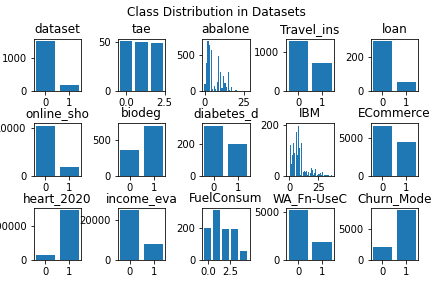
\includegraphics[scale=0.8]{distribution}
	\label{fig:dists}
	\caption{Distribution of the target labels of each file tested.}
\end{figure}

\section{How does feature scaling (i.e. doing standardization) affect the performance?}
To test the effect of standardization on the model performance, we train a \texttt{RandomForest}
classifier with 10 decision trees.
Since we want to measure the effect of standardization on performance
as a whole, we use classification accuracy as our measure.


\begin{table}
\begin{centering}
	\begin{tabular}{|c|c|c|}
	Dataset & Scaled & Non-Scaled \\
	\hline
	Heart Disease & 87.9 & 87.9 \\
	\hline
	Bank Marketing & 88.6 & 87.8 \\
	\hline
	Income Evaluation & 84.8 & 85.1 \\
	\hline
	Telco Customers & 78.3 & 78.8 \\
	\hline
	Abalone & 23.3 & 23.3\\
	\hline
	IBM Attrition & 15.9 & 14.2 \\
	\hline
	Biostar Degradation & 86.6 & 85.5 \\
	\hline
	Credit Card  & 66.2 & 66.6 \\
	\hline
	Fuel Consumption & 80 & 76 \\
	\hline
	Travel Insurance  & 80.6 & 80.7 \\
	\hline
	Diabetes  & 98.4 & 97.6 \\
	\hline
	Loans & 81.2 & 82.0 \\
	\hline
	Onlne Shopper intention & 89.6 & 89.4 \\
	\hline
	Teacher Assistant & 61.3 & 62 \\
	\hline
	Churn Modelling & 85.0 & 84.8\\
	\hline
	\end{tabular}
	\caption{Effects of applying feature standardizaiton.} 
	\label{table:scaling}
\end{centering}
\end{table}

As seen in Table~\ref{table:scaling}, in our experiments feature scaling 
has only a small influence in our accuracy. 
Some datasets such as IBM Attrition and Abalone had poor performance
because there are classes that have only one sample. 
This poses problems when using a \texttt{StratifiedKFold} cross-validation
method.
It is important that we use this evalutation method so we can roughly 
preserve the original distribution of data in each fold.
Most results fall within one percentage point difference between the
standardized and non-standardized approaches.

\section{When using tree-based algorithms, will using one-hot encoding for 
categorical features generate worse performance than label encoding? Why?}
Using one-hot encoding for a RandomForest classifier does indead lead to
worse performance, sometimes by significant amounts.
We run our experiments again using a \texttt{RandomForest} classifier
with 10 decision trees.

One-hot algorithms greatly increase the amount of columns in the dataset.
Tree-based classifiers using an impurity metric such as GINI have a greater
chance of using the new columns in their splits at every stage.
This means that we can end with deep decision trees that rely on these columns.

\begin{table}
\begin{centering}
	\begin{tabular}{|c|c|c|}
	\hline
	Dataset & One-Hot Encoding & Label Encoding \\
	\hline
	Heart Disease & 88.2 & 88.8 \\
	\hline
	Bank Marketing & 86.0 & 87.9 \\
	\hline
	Income Evaluation & 75.8 & 84.6 \\
	\hline
	Telco Customers &75.3 & 78.2\\
	\hline
	Abalone & 21.7 & 22.2\\
	\hline
	IBM Attrition & 10.8 & 15.4 \\
	\hline
	Biostar Degradation & 81.6 & 86.0 \\
	\hline
	ECommerce & 65.7 & 66.1 \\
	\hline
	Fuel Consumption & 56.7 & 78.3 \\
	\hline
	Travel Insurance  & 74.5 & 80.2 \\
	\hline
	Diabetes  & 92.3 & 97.6 \\
	\hline
	Loans & 78.0 & 76.8 \\
	\hline
	Onlne Shopper intention & 85.5 & 89.5 \\
	\hline
	Teacher Assistant & & \\
	\hline
	Churn Modelling &73.8 & 84.7\\
	\hline
	\end{tabular}
	\caption{Effects of applying feature standardizaiton.} 
	\label{table:encoding}
\end{centering}
\end{table}

Table~\ref{table:encoding} shows the results of our encoding experiments.
For the most part, decision trees favor label encoding for categorical features.

\section{Which combinations of numerical and categorical feature transformation methods 
generally lead to better results?}
In this experiment, we test the different combinations of numerical methods and categorical
methods.
We find that there is a difference between different combinations. 
For instance,frequency encoders followed by LightGBM, label encoders with SVM, frequency and LightGBM.
label encoding with random forest are all particularly effective combinations.
MLP encoders might perform comparably to the other methods but often lower when paired with 
other encoders.
The LightGBM pairs are usually quite strong, stronger than xgboost, although ensemble methods
are all very strong performers.

Although ensemble methods and more traditional methods such as SVM perform roughly equal in many 
scenarios, ensemble methods perform well more consistently than these other methods.

\section{If the number of possible categorical values of a feature is high,
which encoding methods among }
To test the relationship of encoding methods and amount of categorical values, 
we try all the encoding methods and see which datasets have the highest possible categorical
values.
Table~\ref{table:p5} shows the results of training a random forest model using three different encoding 
methods.
For One-Hot Encoding, we use a Label Encoder for the target column and apply OHE to the feature columns.
There does not seem to be a large change between the maximum amount of categorical features and the 
overall accuracy.
For instance, using target encoding we can achieve high accuracy with high possible categorical values.
However, since Target Encoding relies on the average of the target values, datasets with many outliers 
in the target column yield lower accuracy. 
For instance, the datasets with lowest accuracy are the IBM and Abalone datasets.
These datasets also have the largest variance in the target column. 
This causes the encoding to not represent the data as accurately.

One Hot Encoding yields the best results by far, even if we are using  a tree-based method.
Since OHE adds columns, we can think of OHE as adding a stronger association between a 1 in certain
columns and the output classification.


\begin{table}
\begin{centering}
	\begin{tabular}{|c|c|c|c|c|}
	\hline
	Dataset & Max Feature Values & target & onehot & label \\
	\hline
	Heart Disease & 13 & 88.9 & 100 & 17 \\
	\hline
	Income Evaluation & 42 & 85.1 & 100 & 84.9 \\
	\hline
	Bank Marketing & 22 & 88.2 & 1.0 & 88.3 \\
	\hline
	Telco Customers & 7043 & 77.5 & 100 & 78.6 \\
	\hline
	Abalone & 3 & 23.9 & 99.8 & 23 \\
	\hline
	IBM Attrition & 6 & 17.3 & 99.7 & 17.1 \\
	\hline
	ECommerce & 5 & 66.1 & 100 & 66.6 \\
	\hline
	Fuel Consumption & 715 & 78.7 & 100 & 75 \\
	\hline
	Travel Insurance  & 2 & 80.8 & 100 & 80.5 \\
	\hline
	Diabetes  & 2 & 97.5 & 100 & 97.8 \\ 
	\hline
	Loans & 23 & 76.8 & 100 & 79.1 \\
	\hline
	Onlne Shopper intention & 10 & 89.5 & 100 & 89.4 \\
	\hline
	Churn Modelling & 2932 & 86.3 & 100 & 84.7 \\
	\hline
	\end{tabular}
	\caption{Accuracy on datasets with different amount of categorical values.}
	\label{table:p5}
\end{centering}
\end{table}


\section{Compare the classification performance of ``doing nothing'', 7 undersampling,
4 oversampling, 2 ensemble-based methods in the presence of class imbalance. Which methods
work generally the best and worst? Why?}

To measure the different types of resampling methods, we go through each file and test the 
over sampling, under sampling, and ensemble samplng methods, along with a control where we do
not perform any resampling.
The performance metric we use is \texttt{sklearn}'s \texttt{precision\_recall\_fscore\_support} metric,
which compares the ground truth values and our predictions and returns these four values.
With further analysis we could find more accurate predictions.

Generally speaking, the \texttt{editedNeuralNearestNeighbors} works best among the undersampling methods, 
while the ovresampling methods tend to achieve higher precision.

\section{Can you find which SMOTE-based oversampling works better on which datasets?}
SMOTE-based oversampling achievies comparable precision results with undersampling methods. 
However, SMOTE-based oversampling does achieve better results on some datasets.
For instance, the diabetes dataset has almost all categorical features. 
All sampling methods perform here across all scores, not only precision.
The income evaluation dataset also has many categorical features, and we find the oversampling 
methods work better on these types of datasets.

Figure~\ref{fig:dists} shows that these two specific datasets are both binary classification tasks
and the degree of imbalance is not as great as the other datasets.

\section{Is a dataset's imbalance ratio (e.g. \%Pos) related to choosing which resampling 
strategy for better performance? Any insights?}
To answer this question, we can see the classes with the highest imbalance in Figure~\ref{fig:dists}.
The Bank Marketing (``dataset'' in Figure~\ref{fig:dists}) has one of the highest signs of imbalance 
among the datasets.
In our experiments this dataset was one of the poorest performers for oversampling methods, 
suggesting that the imbalance ratio plays a large part across the metrics, since all the 
four metrics are much lower.
However, undersampling methods seem less affected by this extreme imabalance.

In the Churn Modelling dataset the imbalance does not seem to affect the performance as much as the 
Bank Marketing dataset, although all the metrics are lower across the board compared to less imbalanced
datasets.
The precision on the Churn Modelling dataset is slightly lower among the oversampling methods compared 
to undersampling methods.
The recall among the undersampling methods suggests that undersampling methods might be more effective 
when there are extreme imbalances in data, while both approaches are comparable in less extrmeme 
scenarios.

\section{How do different ML algorithms (Random Forest, XGBoost, LightGBM, MLP, SVM) prefer different
resampling strategies for better performance of imbalance classification?}
Ensemble methods such as Random Forest and XGBoost, which rely on minimizing the impurity in splits.
For these methods, methods such as Neighborhood Cleaning Rule method can remove the 
points right along the decision border that could lead to decreased performance.
A mitigating factor could be that with many random forests the effects of imbalance could be mitigated a 
little.
High-dimensional methods also would benefit from ensemble methods which, at the cost of increased training time, 
address the main issues of SMOTE-based oversampling methods.

Multi-Layer Perceptrons are useful for high dimensional inputs, and could learn a more fine-grained 
decision boundary for points that are on the decision boundary.
The nearmiss undersampling method could help increase the linear separability by removing the closest $k$
majority class samples. 
This could highlight the difference among the majority of the class samples, helpful to SVM.

\section{Conclusion}
In this assignment we considered many different feature encoding and sampling methods.
The objective of these methods is to elminate some of the uncertainty and unpredictability 
that often happen when sampling data.
We considered the different scenarios, combinations, and use cases where these methods can be 
useful for us.
While there is no ``best'' method, different factors, e.g. imbalance ratio, can affect the best
choice of encoder and sampling method across datasets.
Another finding is that more ``complex''or newer methods are not always better. 
XGBoost, which has become a very popular ensemble method in recent years, does not perform 
universally better than a simpler method such as SVM.

This assignment was useful in allowing us to explore the combinations of encoding methods which 
are not often taught.
Although getting such different encoders and samplers to work uniformly on every dataset required
much work, it is still a very useful excercise, especially for future projects where we run into 
imbalanced data or categorical data.
\end{document}
